%-------------------------
% Resume in Latex
% Author : Arya veer Singh chauhan
%------------------------

\documentclass[letterpaper,10pt]{article}
\usepackage{multirow}
\usepackage{latexsym}
\usepackage[empty]{fullpage}
\usepackage{titlesec}
\usepackage{marvosym}
\usepackage[usenames,dvipsnames]{color}
\usepackage{verbatim}
\usepackage{enumitem}
\usepackage[dvipsnames]{xcolor}
\usepackage[hidelinks]{hyperref}
\usepackage{fancyhdr}
\usepackage[english]{babel}
\usepackage{tabularx}
\usepackage{hyphenat}
\usepackage{fontawesome}
\usepackage{float}
\usepackage{tikz}
\usepackage{graphicx}
\usepackage[
top    = 0.5cm,
bottom = 0.5cm,
left   = 0.5cm,
right  = 0.5cm]{geometry}

%---------- FONT OPTIONS ----------
% sans-serif
% \usepackage[sfdefault]{FiraSans}
% \usepackage[sfdefault]{roboto}
\usepackage[sfdefault]{noto-sans}
% \usepackage[default]{sourcesanspro}

% serif
% \usepackage{CormorantGaramond}
% \usepackage{charter}


\pagestyle{fancy}
\fancyhf{} % clear all header and footer fields
\fancyfoot{}
\renewcommand{\headrulewidth}{0pt}
\renewcommand{\footrulewidth}{1pt}

\usepackage{xpatch}
\xapptocmd{\footrule}{\color{Cerulean}}{}{}
\xpretocmd{\footrule}{\color{Cerulean}}{}{}

% Adjust margins
%\addtolength{\oddsidemargin}{-0.8in}
%\addtolength{\evensidemargin}{-0.8in}
%\addtolength{\textwidth}{1.4in}
%\addtolength{\topmargin}{-.8in}
%\addtolength{}
%\addtolength{\textheight}{0.4in}

\urlstyle{same}

\raggedbottom
\raggedright
\setlength{\tabcolsep}{0in}


% Sections formatting
\titleformat{\section}{
  \vspace{-7pt}\scshape\raggedright\large
}{}{0em}{}[\color{Cerulean}\titlerule \vspace{-4pt}]

% Ensure that generate pdf is machine readable/ATS parsable
\pdfgentounicode=1

%-------------------------
% Custom commands

\newcommand{\resumeItem}[1]{
  \item\small{
    {#1 \vspace{-2pt}}
  }
}


\newcommand{\resumeSubheading}[4]{
  \vspace{-2pt}\item
    \begin{tabular*}{0.97\textwidth}[t]{l@{\extracolsep{\fill}}r}
      \textbf{#1} & #2 \\
      \textit{\small#3} & \textit{\small #4} \\
    \end{tabular*}\vspace{-7pt}
}


\newcommand{\resumeSubSubheading}[2]{
    \vspace{-2pt}\item
    \begin{tabular*}{0.97\textwidth}{l@{\extracolsep{\fill}}r}
      \textit{\small#1} & \textit{\small #2} \\
    \end{tabular*}\vspace{-7pt}
}


\newcommand{\resumeEducationHeading}[4]{
  \vspace{-2pt}\item
    \begin{tabular*}{0.97\textwidth}[t]{l@{\extracolsep{\fill}}r}
      \textbf{#1} & #2 \\
      \textit{\small#3} & \textit{\small #4} \\
    \end{tabular*}\vspace{-5pt}
}


\newcommand{\resumeProjectHeading}[2]{
    \vspace{-2pt}\item
    \begin{tabular*}{0.97\textwidth}{l@{\extracolsep{\fill}}r}
      \small#1 & \small#2 \\
    \end{tabular*}\vspace{-7pt}
}

\newcommand{\resumeOrganizationHeading}[3]{
  \vspace{-2pt}\item
    \begin{tabular*}{0.97\textwidth}[t]{lr}
      \textbf{#1} & \textit{\small #2} \\
      \textit{\small#3}
    \end{tabular*}\vspace{-7pt}
}

\newcommand{\resumeProfile}[6]{
		\begin{minipage}{0.2\linewidth}
			\frame{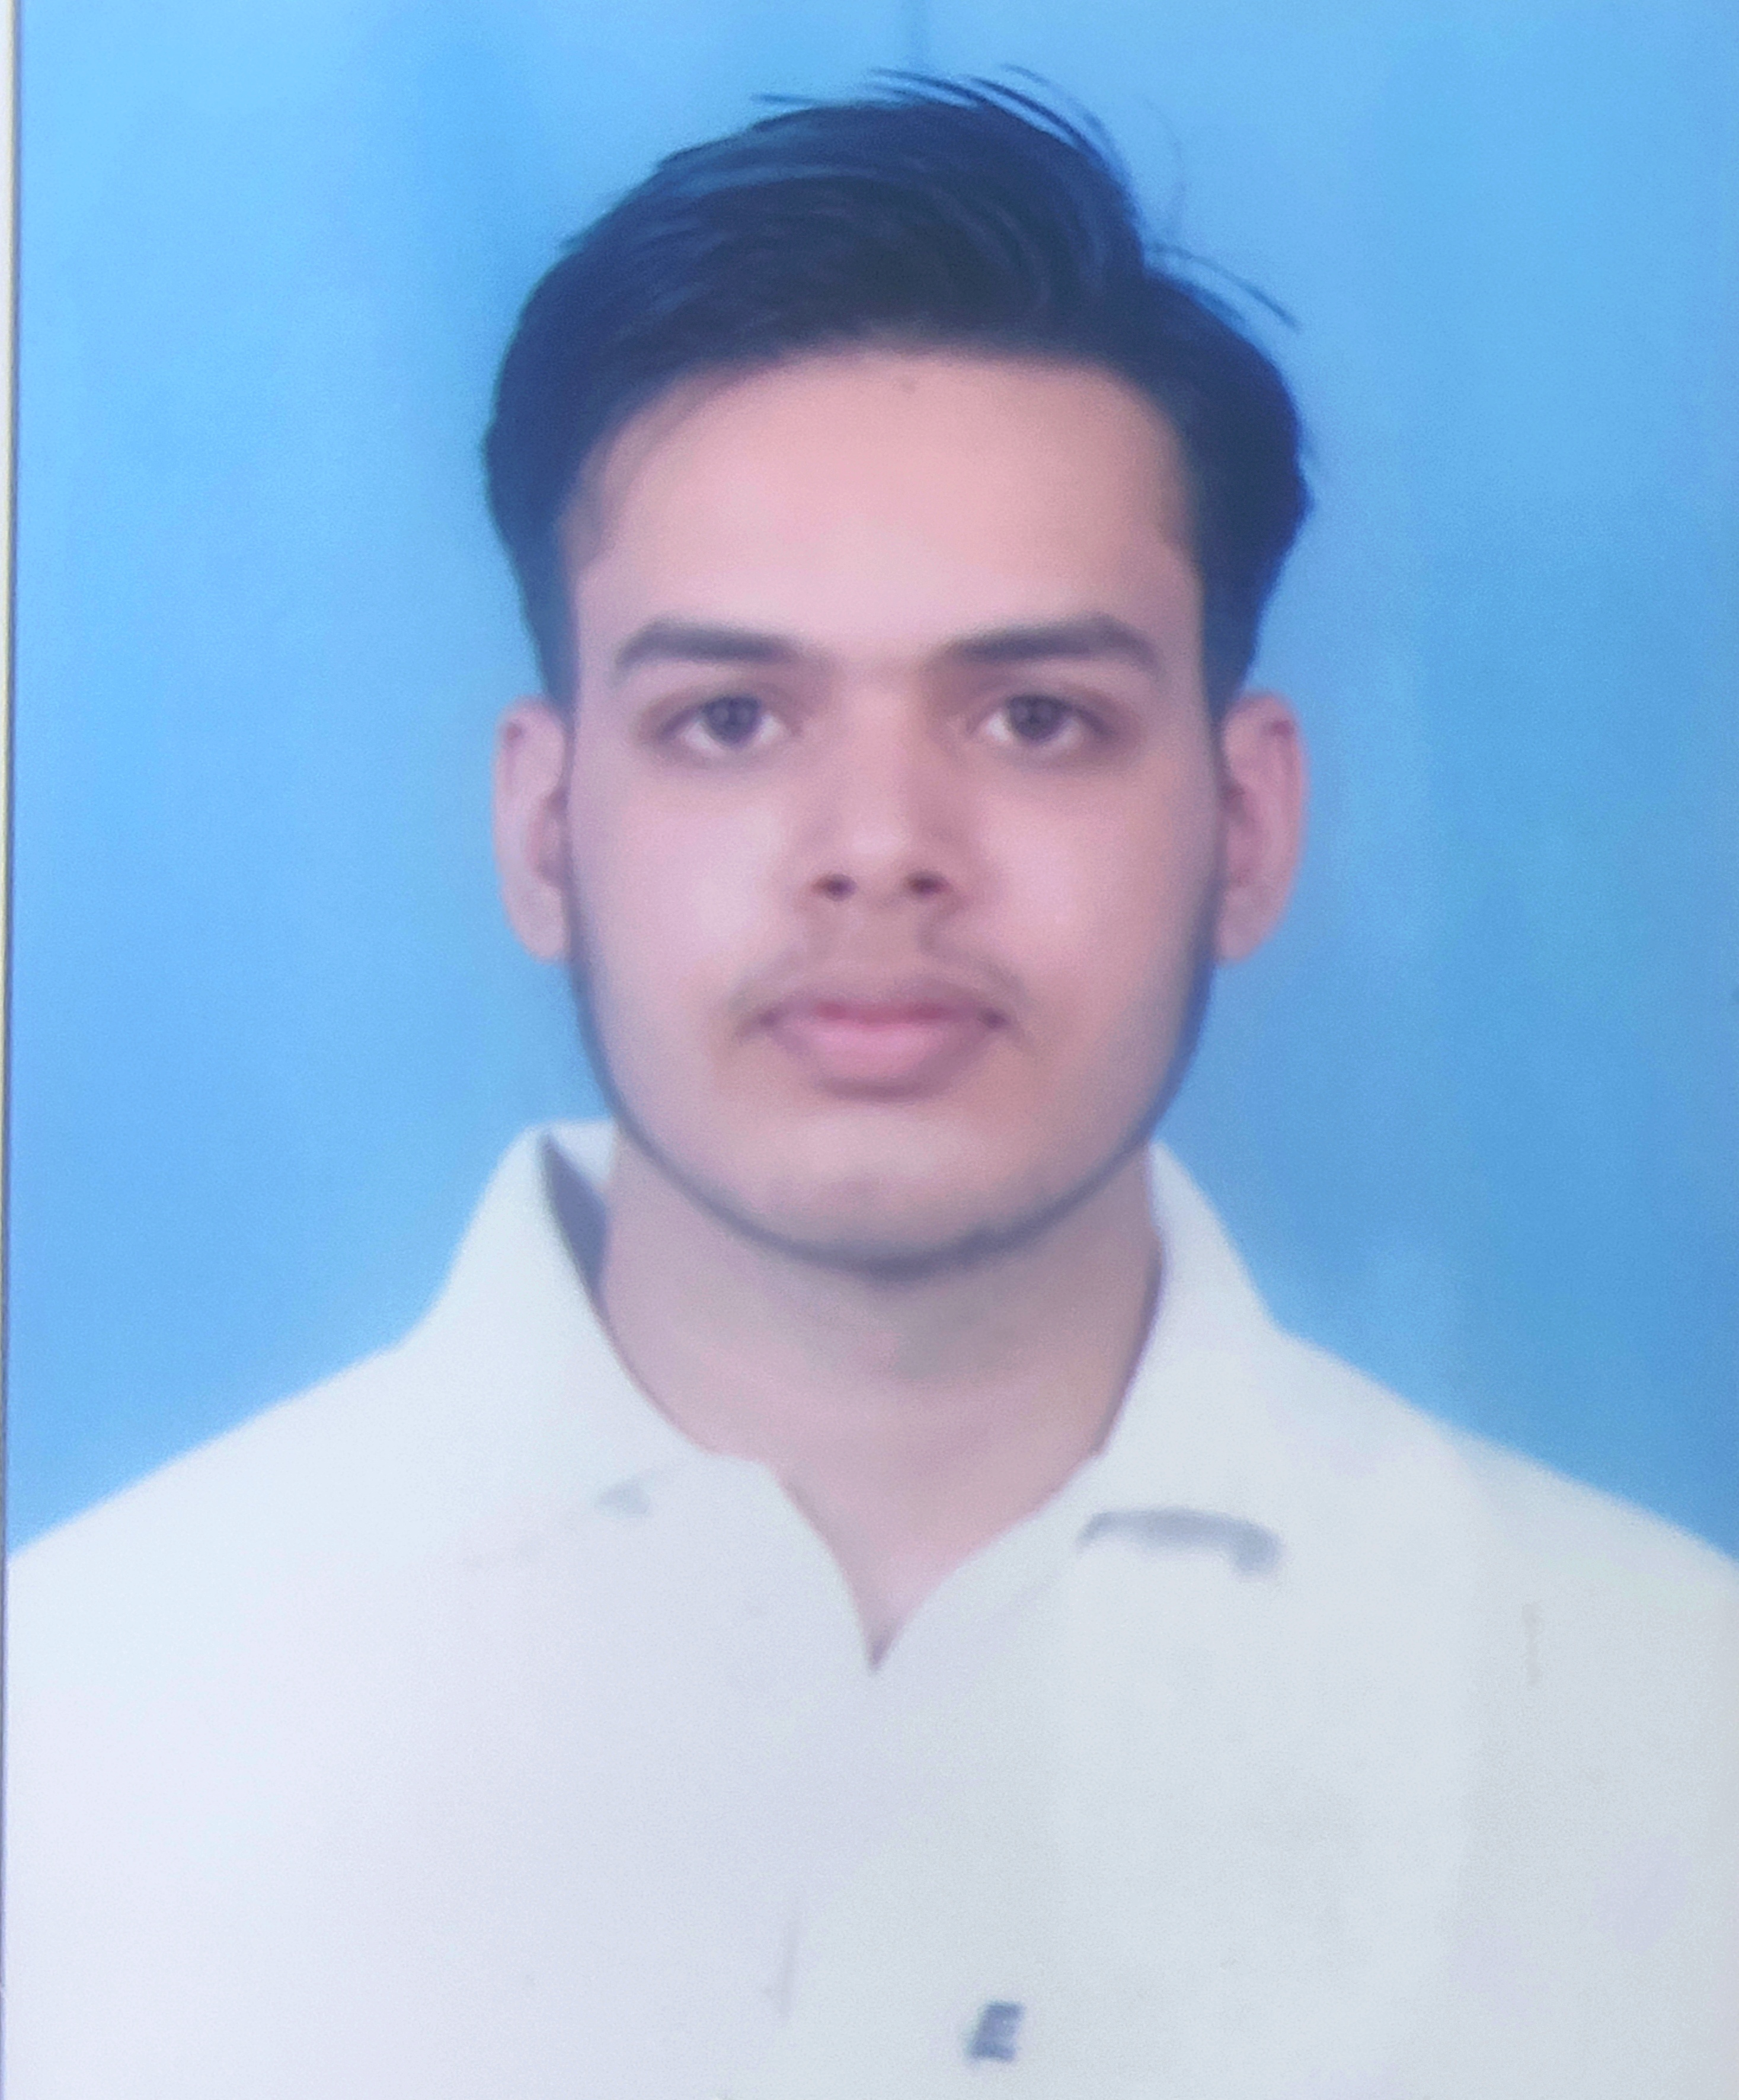
\includegraphics[width=.6\linewidth]{profile.jpg}}
		\end{minipage}
		\begin{minipage}{0.78\textwidth}\raggedright
			\begin{flushright}
				{\textbf{\Huge \scshape #1}}\\ \vspace{6pt}
				\large
				\color{Cerulean}$|$\color{black}
				\hspace{0.3pt}
				\faMobile \hspace{.5pt} \href{tel:+91{#2}}{+91 {#2}}
				\color{Cerulean}$|$\color{black}
				\hspace{0.3pt}
				\faAt \hspace{.5pt} \href{mailto:{#3}}{#3}
				\\ \vspace{2pt}
				\hspace{0.3pt}
				\faLinkedinSquare \hspace{.5pt} \href{#4}{LinkedIn} 
				\hspace{0.3pt} 
				\faGithub \hspace{.5pt} \href{#5}{GitHub}
				\hspace{0.3pt}
				\faGlobe \hspace{.5pt} \href{#6}{Portfolio}
			\end{flushright}
		
		\end{minipage}
		\noindent
		\\ \vspace{8pt}
}

\newcommand{\resumeSubItem}[1]{\resumeItem{#1}\vspace{-4pt}}

\renewcommand\labelitemii{$\vcenter{\hbox{\tiny$\bullet$}}$}

\newcommand{\resumeSubHeadingListStart}{\begin{itemize}[leftmargin=0.15in, label={}]}
\newcommand{\resumeSubHeadingListEnd}{\end{itemize}}
\newcommand{\resumeItemListStart}{\begin{itemize}}
\newcommand{\resumeItemListEnd}{\end{itemize}\vspace{-5pt}}

%-------------------------------------------
%%%%%%  RESUME STARTS HERE  %%%%%%%%%%%%%%%%%%%%%%%%%%%%


\begin{document}

%---------- HEADING ----------

\resumeProfile{ARYA VEER SINGH CHAUHAN}{8619151680}{aryaveersingh2003@gmail.com}{https://www.linkedin.com/in/arya-veer-singh-chauhan-428154210/}{https://github.com/Arya-veer}{https://arya-veer-portfolio.vercel.app/}



%----------- EDUCATION -----------

\section{Education}
  \vspace{3pt}
  \resumeSubHeadingListStart
    \resumeEducationHeading
      {Birla Institute of Technology and Science, Pilani}{Pilani, India}
      {B.E. Computer Science Engineering;   \textbf{GPA: 8.64/10}}{2020 \textbf{--} 2024}
    \resumeSubHeadingListEnd

%----------- SKILLS -----------

\section{Skills}
  \vspace{2pt}
  \resumeSubHeadingListStart
    \small{\item{
        \textbf{Languages:}{ C/C++, Java, Python, JavaScript, SQL, NASM} \\ \vspace{3pt}
        \textbf{Technologies:}{Django, Django Rest framework, React.js, Next.js, MySQL, Postgresql, Spring Boot, Postman, Compiler construction, Server Configuration, Socket Programming, Git, SVN, Docker, AWS, Kubernetes, GCP, Kafka, RabbitMQ} \\ \vspace{3pt}
        \textbf{Methodologies:}{ Agile, Scrum, OOP, Functional Programming, Microservices, API Testing automation, Design Patterns} \\ \vspace{3pt}
    }}
  \resumeSubHeadingListEnd



%----------- EXPERIENCE -----------

\section{Experience}
  \vspace{3pt}
  \resumeSubHeadingListStart

  \resumeSubheading
  {BITS Pilani Library}{Pilani, India}
  {Software Developer}{August 2023\textbf{--} May 2024, Part-time}
    \resumeItemListStart
        \resumeItem{Digitalised the heritage gallery of BITS having 1000+ media files developing \color{Cerulean}\href{https://library.bits-pilani.ac.in/bhg/}{heritage website} \color{black} using \textbf{React.js} and \textbf{MongoDB}.}
        \resumeItem{Designed and Programmed the \color{Cerulean}\href{https://library.bits-pilani.ac.in}{official library website} \color{black} of BITS utilising \textbf{Next.js} for server-side rendering and \textbf{Django} for backend.} 
        \resumeItem{Conceptualized a framework using \textbf{multithreading} to upload data \textbf{asynchronously}. Reduced data upload request time by 85\%}
    \resumeItemListEnd

    \resumeSubheading
      {Standard Chartered GBS}{Bengaluru, India}
      {SDE Intern}{May, 2023 \textbf{--} July, 2023}
        \resumeItemListStart
            \resumeItem{Engineered a proof-of-concept software with \textbf{React.js} and \textbf{Spring Boot} for reducing manual work by 4 hours in account opening.}
            \resumeItem{Enhanced the core functionality of utility library to compare two XML files using \textbf{Java} and tested the same using \textbf{JUnit}.}
            \resumeItem{Pipelined API development, documentation and testing through \textbf{postman} automated with \textbf{newman} and python subprocesses.}
        \resumeItemListEnd
    
  \resumeSubHeadingListEnd



%----------- AWARDS & ACHIEVEMENTS -----------


%----------- PROJECTS -----------

\section{Projects}
    \vspace{3pt}
    \resumeSubHeadingListStart

      \resumeProjectHeading{\textbf{Studydeck}}{July 2023 - October 2024}
	   	  \resumeItemListStart
	  	    \resumeItem{Created the backend using \textbf{Django} for a platform-independent software used by more than 80\% BITS students for the academics.}
	  	    \resumeItem{Devised a \textbf{BFS} and \textbf{multithreading} based algorithm to parse google drive and store 800 GB of study resources in \textbf{S3 bucket}.} 
	  	    \resumeItem{Consolidated a \textbf{CDN} on campus LAN to decrease approx. 70\% cost and also provided a resource-sharing feature to students.}
	  	    \resumeItem{Automated timetable download and parsing to prepopulate database, and allowing students to customize their own timetables.} 
	  	    \resumeItem{Empowered the feature with autocomplete having a \textbf{backtracking-based algorithm} in \textbf{C++} to increase code efficiency 20 times.}
	   	  \resumeItemListEnd

      \resumeProjectHeading{\textbf{ERPLAG Compiler}}{Feb 2023 - May 2023}
        \resumeItemListStart
          \resumeItem{Architected a compiler in \textbf{C} for given specifications implementing lexical and syntax analyzer to check for errors during compile time. Generated a parse tree using data structures like \textbf{Linked List}, \textbf{Stack} and \textbf{Hash map}. Integrated panic-mode error recovery.}
          \resumeItem{Implemented the backend of compiler with Abstract Syntax Tree reducing memory efficiency by 70\% for semantic analysis.}
          \resumeItem{Established a three-address code technique to convert the given code into \textbf{NASM} assembly code for execution and runtime checks.}
        \resumeItemListEnd

      \resumeProjectHeading{\textbf{Project Onetap}}{September 2021 - March 2022}
          \resumeItemListStart
            \resumeItem{Formulated a system providing services to 8000+ college students developing multiple softwares and integrating them together.}
            \resumeItem{Provided \textbf{REST APIs} to mobile applications and a desktop application for a food ordering and delivering service using \textbf{Python}.} 
            \resumeItem{Implemented an encrypted QR-based wallet using \textbf{Symmetric encryption}, and facilitated secure transactions over Rs. 10 cr. p.a.}
            \resumeItem{Built a web application using \textbf{React.js} and \textbf{Django} for booking, functioning and monitoring of cab service in campus deployed \color{Cerulean}\href{https://cab-admin.su-bitspilani.org}{here}}
          \resumeItemListEnd

    \resumeSubHeadingListEnd


%----------- THESIS -----------
\section{Bachelor's Thesis}
	\vspace{3pt}
	\resumeSubHeadingListStart
		\resumeProjectHeading{\textbf{Title: Design and Implementation of Software Systems to Support Big Data and AI Techniques in Disease Diagnosis} \\
		\small Supervisor: \href{mailto: tanmay.mahapatra@pilani.bits-pilani.ac.in}{Dr. Tanmay Mahapatra}
		}{}
			\resumeItemListStart
				\resumeItem{Deciphered the underlying software architecture of 10 solutions across world to understand the features and limitations in them.}
				\resumeItem{Conceptualized an Indian context based architecture to solve the EHR collection problem to provide datasets for medical research.}
				\resumeItem{Deployed the pilot implementation as a web-application developed using \textbf{Django},\textbf{React.js} and \textbf{postgresql} having SUS score of 72.9}
			\resumeItemListEnd
	\resumeSubHeadingListEnd
		
	

%----------- RELEVANT COURSEWORK -----------

 \section{Coursework}
 	\vspace{2pt}
 	\resumeSubHeadingListStart
 		\small{\item{
 				C Programming, \textbf{Object-oriented programming(Class topper)}, Discrete Structures, Database Systems, Data Structures and Algorithms, Operating Systems, Computer Architecture, Principles of programming languages, Computer Networks, Compiler Construction, Artificial Intelligence, Design and Analysis of Algorithms 
 				 \\ \vspace{3pt}
 		}
 				}
 	\resumeSubHeadingListEnd



	

%----------- ORGANIZATIONS -----------

% \section{Organizations}
%   \resumeSubHeadingListStart   
%     \resumeOrganizationHeading
%       {Students' Union Technical Team (SUTT)}{Feb 2021 -- Present}{Student Member}
%   \resumeSubHeadingListEnd



%----------- HOBBIES -----------

% \section{Hobbies}
  % \resumeSubHeadingListStart
    % \small{\item{Basketball, Swimming, Fitness, Eight-ball, Horology}}
  % \resumeSubHeadingListEnd



%----------- REFERENCES -----------

% \section{References}
  % \vspace{2pt}
  % \resumeSubHeadingListStart
    % \item{References available upon request.}
  % \resumeSubHeadingListEnd



%-------------------------------------------
\end{document}